% ! TeX root = ../../../master-thesis.tex

\subsection{ScaFi}
\label{section:background:technologies:scafi}

\textbf{\ac{ScaFi}}\footnote{Repository at: \url{https://github.com/scafi}} is an
open-source aggregate computing framework for the Scala programming language,
providing a usable internal \ac{DSL} for aggregate specifications and a
platform for the simulation and execution of such specifications
\cite{ScaFi-Documentation}.

In \ac{ScaFi}, the core concepts of field calculus are modelled by a
\textbf{trait} (i.e., an interface) like the one reported in Listing
\ref{listing:scafi-field-calculus} \cite{FieldCalculus-AggregateComputing},
whose methods represent the constructs of field calculus.

\lstinputlisting[
  language=Scala,
  caption={The core constructs of field calculus, represented as a trait,
      abstracting over the actual organization within ScaFi.},
  captionpos=b,
  label={listing:scafi-field-calculus}
]{resources/listings/scafi-field-calculus.txt}

\ac{ScaFi} provides no explicit reification for computational fields. Indeed,
any Scala expression is treated implicitly as a field calculus expression,
yielding a computational field. For instance, the expression \enquote{$1+2$}
yields constant uniform computational field holding the value $3$ at any point
in space and time, obtained as the point-wise summation of a field of
\enquote{$1$}s and a field of \enquote{$2$}s (Figure
\ref{figure:constant-uniform-field}).

\begin{figure}[h]
  \centering
  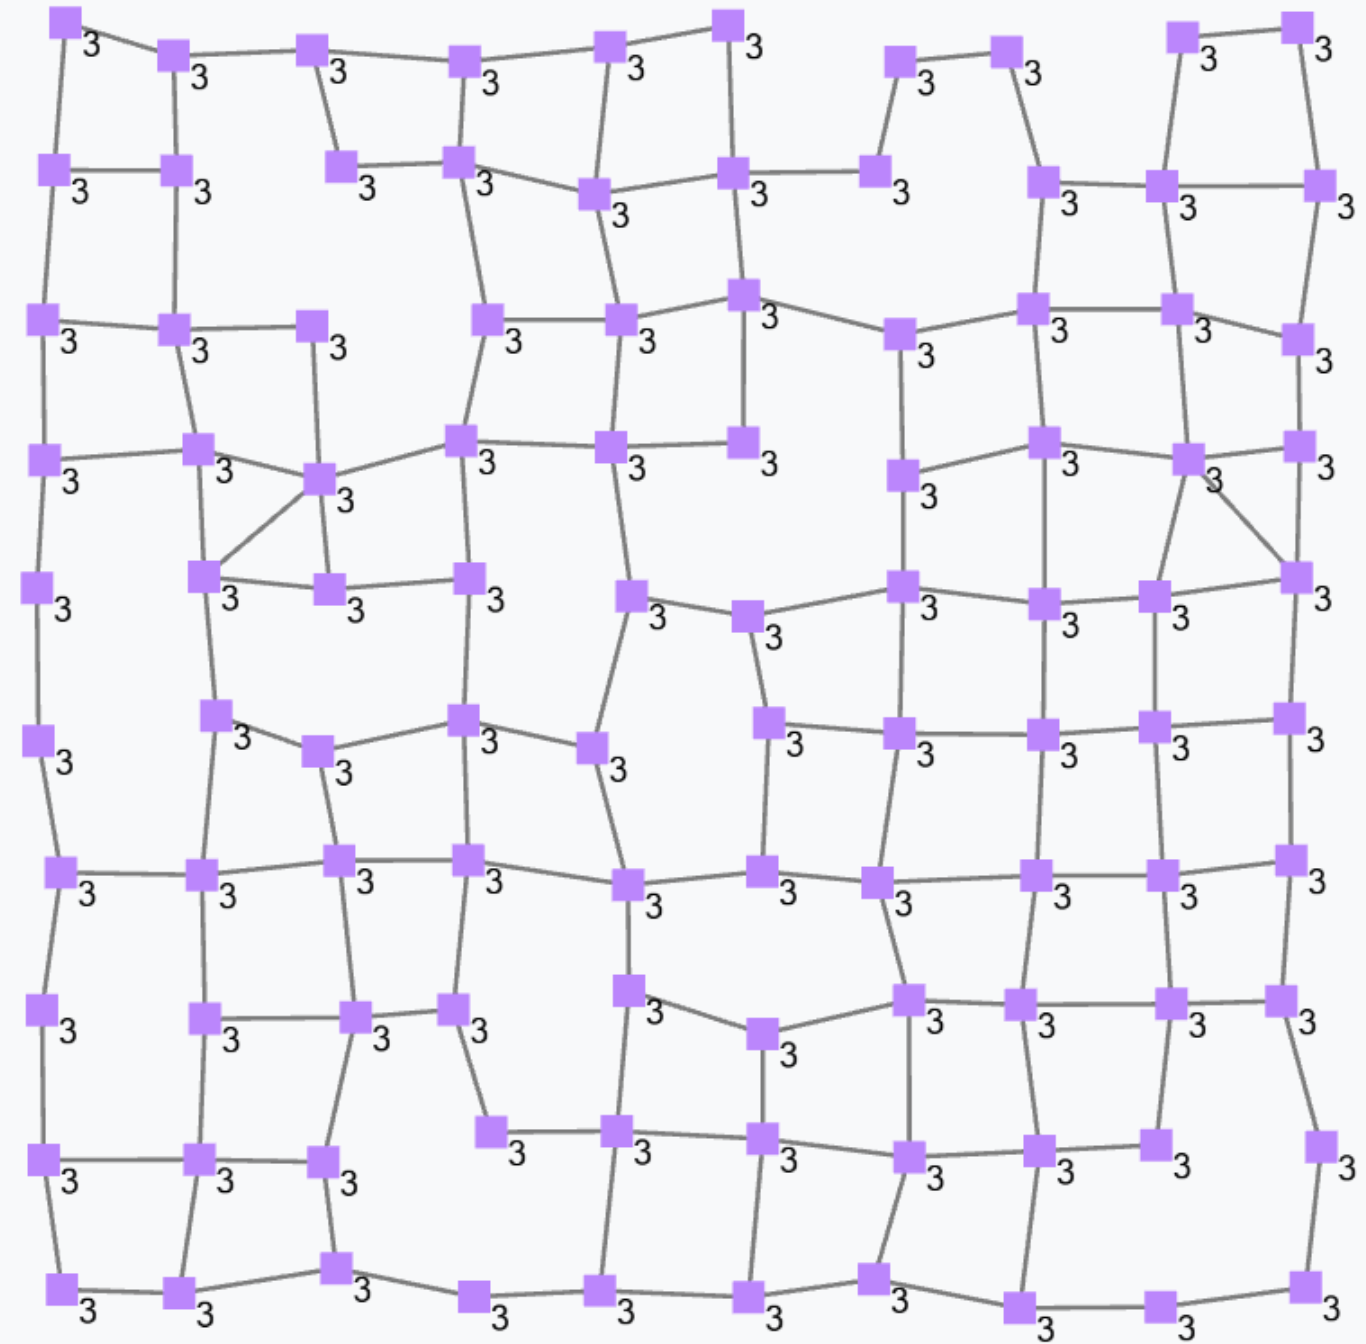
\includegraphics[width=0.55\textwidth]{resources/figures/constant-uniform-field.png}
  \caption{
    A graph representing an aggregate of devices (\textit{nodes}) and their
    neighbouring relations (\textit{edges}). In particular, it represents the
    computational field yielded by the expression \enquote{$1+2$}
    (image from the site \cite{ScaFi-Documentation}).
  }
  \label{figure:constant-uniform-field}
\end{figure}

Despite being equivalent, the semantics of \ac{ScaFi} differs from the
semantics of field calculus for some operators: evolution over space is
implemented with a combination of the \texttt{nbr} and \texttt{foldhood}
operators, the latter exploiting the former to accumulate the values of
neighbours in each device (i.e., \texttt{nbr} does not yield a neighbouring
value directly as in field calculus); restriction is implemented using the
\texttt{aggregate} operator, which handles selective partitioning; evolution
over time with \texttt{rep} follows the same semantics as in field calculus.

Additionally, \ac{ScaFi} provides contextual operators that handle interactions
with the underlying platform, namely \texttt{mid}, which computes the field of
the device identifiers, \texttt{sense}, which computes a field of the values
perceived by a specific sensor from the environment (e.g., a field of
temperatures), and \texttt{nbrvar}, which computes a field mapping each
neighbour to a value perceived by a specific sensor from the environment (e.g.,
a field of distances with each neighbour).

The core \ac{DSL} can be extended with \textbf{mixins} to provide higher-level
primitives and operators. \ac{ScaFi} already includes some built-in extensions,
such as the resilient aggregate computing blocks (Listing
\ref{listing:scafi-aggregate-computing}).

\lstinputlisting[
  language=Scala,
  caption={The core constructs of aggregate computing, represented as a mixin
      for field calculus, abstracting the actual organization within ScaFi.},
  captionpos=b,
  label={listing:scafi-aggregate-computing}
]{resources/listings/scafi-aggregate-computing.txt}

The higher-level primitives in \ac{ScaFi} include but are not limited to the
already presented \texttt{G}, \texttt{C} and \texttt{T} blocks of aggregate
computing, an additional \texttt{S} block, which handles sparse leader election
based on proximity, a \texttt{branch} operator, implementing the branching
expression of field calculus (relying on
\texttt{aggregate})\footnote{Conditional computation without partitioning is
implemented by the \texttt{mux} operator instead, which is equivalent to an
\textit{if-then-else} expression in Scala.}, and a new \texttt{share} operator,
which handles the evolution over time of a neighbouring value (indeed a
combination of the behaviours of \texttt{rep} and \texttt{nbr} in field
calculus, albeit much more efficient \cite{ScaFi-ShareOperator}).

The execution of a \ac{ScaFi} specification is performed by the underlying
platform, which adopts an \textit{asynchronous} \textbf{round-based} execution
model, in which a round is the computation required for an individual device to
produce its next output based on the aggregate specification. A round consists
of the following three steps in order:
\begin{enumerate}
  \item \textbf{sense}: the device updates its current \textbf{context} (i.e.,
        all known information from its perspective), by retrieving its previous
        output, the information perceived through its \textit{sensors} from the
        local environment and the messages transmitted by neighbouring devices.
  \item \textbf{compute}: the device computes its current output by executing
        the aggregate specification against its current context. The output of
        a device is an abstract syntax tree, tracking the structure of the
        executed aggregate specification for alignment. In particular, the root
        of the tree contains the final result of the computation, while the
        roots of its subtrees contain the results of sub-computations.
  \item \textbf{interact}: the device broadcasts some information extracted
        from its output (called an \textbf{export}) to neighbouring devices and
        updates the local environment through its \textit{actuators}. The
        export can be derived from the output of the device by searching in the
        abstract syntax tree for operations involving communication (e.g.,
        subtrees depending on \textbf{nbr}).
\end{enumerate}

Support for simulation is also implemented by several \ac{ScaFi} modules or
through integration with third-party simulators (e.g.,
Alchemist\footnote{Repository at:
\url{https://github.com/AlchemistSimulator/Alchemist}} \cite{Alchemist}).
